\documentclass[11pt,a4paper]{article}
\usepackage[utf8]{inputenc}\usepackage[T1]{fontenc}
\usepackage[margin=1in]{geometry}
\usepackage{amsmath,amssymb,booktabs,graphicx,enumitem,xcolor,parskip,titlesec}
\usepackage[hidelinks]{hyperref}
\graphicspath{{figures/}}
\definecolor{qnavy}{RGB}{20,40,75}\definecolor{qgrey}{RGB}{90,90,90}\definecolor{qred}{RGB}{150,30,30}
\titleformat{\section}{\large\bfseries\color{qnavy}}{\thesection}{0.6em}{}
\begin{document}\thispagestyle{empty}
\noindent
{\large\bfseries\color{qnavy} Report R07 --- Methylation and EGFR-TKI Response}\\[2pt]
{\color{qgrey}GSE147377, $n=79$. An inconclusive result, reported as inconclusive rather than
as a negative finding.}\\[6pt]
{\color{qgrey}\rule{\textwidth}{0.4pt}}

\medskip
\noindent 7 August 2026 \quad\textbullet\quad Quantara

\section*{Summary}

This is the only cohort in our holdings that pairs genome-wide DNA methylation with a
\emph{treatment-response} endpoint, and so it is the closest available test of the question the
withdrawn lung manuscript was actually asking. It is also small: 79 advanced lung
adenocarcinoma patients, all EGFR-TKI treated, of whom 40 achieved partial response, 29
progressed and 10 were stable.

Cross-validated elastic-net logistic regression over 464{,}994 complete probes gives
\textbf{AUROC 0.555 (95\% CI 0.42--0.69)} for distinguishing progression from partial response.
A 100-fold permutation null was centred correctly at 0.491 and the observed value sits inside
it ($p=0.30$). There is no detectable methylation signal for TKI response here.

\textbf{The important caveat runs the other way from the usual one.} A power calculation on
this cohort gives a minimum detectable AUROC of \textbf{0.685} at 80\% power. Anything weaker
than that was invisible by construction. So this result does \emph{not} license the statement
``methylation does not predict TKI response'' --- it licenses only ``if such a signal exists
and is of moderate strength or less, this cohort could not have seen it.'' The run artefact's
\texttt{\_decision} field is worded as ``no evidence''; \S4 records why the report states the
weaker and correct claim instead.

\section{The mapping problem, and how it was settled}

The supplementary beta matrix labels its columns \texttt{EXP\_1}\,\ldots\,\texttt{EXP\_79}, not
GSM accessions. Joining methylation to phenotype therefore rests on an assumption --- that
matrix column order matches series-matrix sample order --- and a silent mis-mapping would have
invalidated every number in this report while still producing plausible-looking output. Two
positive controls were pre-registered to test it.

\begin{center}
\begin{tabular}{@{}llll@{}}
\toprule
\textbf{Control} & \textbf{Prediction} & \textbf{Observed} & \textbf{Verdict} \\
\midrule
A. AHRR \texttt{cg05575921} & smokers lower & 0.641 vs 0.702, $p=0.093$ &
  direction correct, underpowered \\
B. Sex separability & a probe near-perfect & \texttt{cg04744025}, AUROC $=1.000$ &
  \textbf{decisive} \\
\bottomrule
\end{tabular}
\end{center}

Control B settles it. With 46 female and 33 male samples, a single probe separating the sexes
perfectly by chance has probability $1/\binom{79}{33} \approx 5\times10^{-23}$; across the
20{,}000 probes screened, the expected number of chance-perfect separations is
$\sim\!10^{-18}$. Observing one is only possible if the sample mapping is correct.

Control A points the same way but does not reach significance. Its direction is right --- median
beta 0.641 in smokers against 0.702 in never-smokers, the established direction for this
biomarker --- and the shortfall is explained by cohort composition: 55 of 79 patients are
never-smokers, which is expected for an EGFR-mutant series but leaves only 24 smokers, and the
label does not distinguish current from former or light from heavy. This is a power limitation
of the control, not evidence against the mapping.

\begin{center}
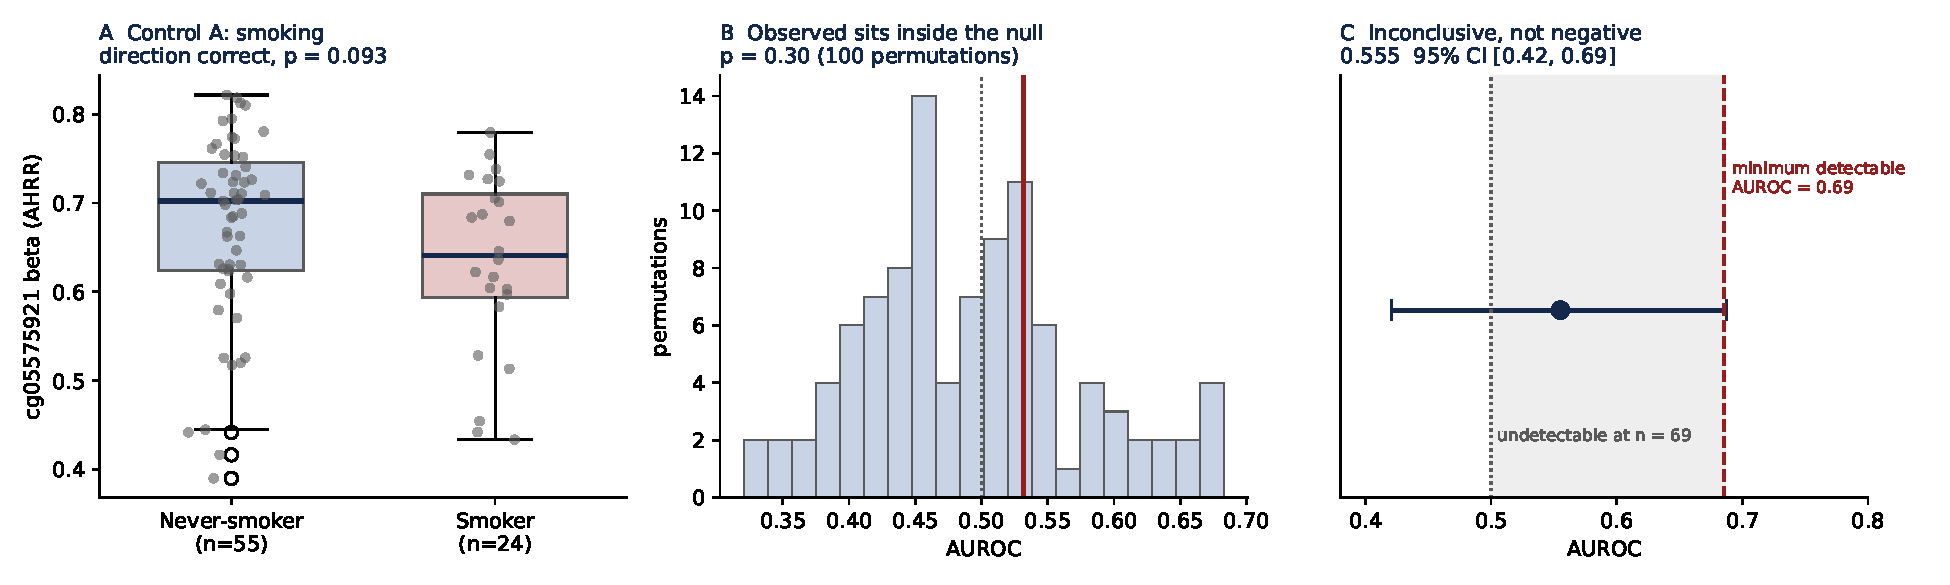
\includegraphics[width=\textwidth]{r07_panels.pdf}
\end{center}
\noindent{\small\color{qgrey}\textbf{A} The AHRR smoking control: correct direction,
$p=0.093$. \textbf{B} The observed cross-validated AUROC (red) against its permutation null;
the null is centred at 0.491, confirming no leakage. \textbf{C} The observed AUROC with its
bootstrap interval; the shaded band is the region this cohort had no power to detect.}

\section{Primary analysis}

Progression (29) versus partial response (40); the 10 stable-disease patients were excluded in
advance as an ambiguous class. Features were the 464{,}994 probes with no missing values across
these 69 patients. Probe selection and hyperparameter choice were performed strictly inside
training folds, in $10\times$ repeated 5-fold nested cross-validation.

\begin{center}
\begin{tabular}{@{}lr@{}}
\toprule
Patients (PR / PD) & 69 (40 / 29) \\
Probes used & 464{,}994 \\
AUROC, pooled out-of-fold & 0.555 \quad 95\% CI 0.42--0.69 \\
AUROC, mean of 10 repeats & 0.532 $\pm$ 0.039 \\
Permutation null mean & 0.491 \\
Permutation $p$ (like-for-like) & 0.30 \\
Minimum detectable AUROC, 80\% power & 0.685 \\
\bottomrule
\end{tabular}
\end{center}

The gap between the pooled figure (0.555) and the mean across repeats
(0.532) is the expected effect of averaging predicted probabilities over repeats. Both are
reported; the second is the one compared against the null, for the reason in \S4.

\section{Audit}

Three findings, all recorded in \texttt{evidence/audit\_addendum.json}.

\textbf{4.1 A gate fired incorrectly on the first run, and was corrected in the script rather
than waived.} The pre-registered rule reads: \emph{``if neither control holds, the mapping is
wrong and no response result is reported.''} The first implementation gated on control A alone
and halted the run when it returned $p=0.093$. That halt was a coding error --- the rule is a
disjunction --- not a real failure. The fix evaluates both controls and halts only if both
fail. Both runs are retained: \texttt{evidence/gates\_FIRST\_HALTED\_RUN.json} is the halted
one. The correction was made to match the pre-registered rule, and the rule itself was not
edited; its wording is fixed by the config hash of the first run.

\textbf{4.2 The originally reported permutation $p$ was anti-conservative, and has been
corrected upward.} The observed statistic was the AUROC of probabilities averaged over 10
repeats, while each null replicate was a single 5-fold split. Averaging reduces variance and
raises AUROC, so the two were not comparable and the comparison favoured significance. Recast
like-for-like --- mean per-repeat AUROC 0.532 against the same null --- the $p$-value moves from
0.188 to \textbf{0.297}. The correction moves away from significance, so the conclusion is
unaffected; the report quotes 0.30.

\textbf{4.3 The conclusion is bounded by power, not by the data.} The pre-registration
declared this cohort underpowered, and the analysis confirms how severely: 40 versus 29
patients cannot resolve an AUROC below 0.685 at conventional power. The confidence interval,
0.42--0.69, is consistent with no effect and equally consistent with a moderate one. Reporting
this as a negative finding would overstate it, so the summary states the bounded claim. For
contrast, the negative control behaved exactly as it should --- the permutation null is centred
at 0.491, so the pipeline is not leaking --- which is what allows the result to be read as
genuinely uninformative rather than broken.

\section{What this means for the lung arm}

Taken with R06, the position on lung is:

\begin{itemize}[leftmargin=1.2em,itemsep=2pt]
\item \textbf{Prognosis from mutation data is tractable and was measured.} R06 found KEAP1
(HR 2.07, $q<0.0001$) and SMARCA4 (HR 1.73, $q=0.0009$) associated with shorter overall
survival in 1{,}127 patients, with both positive controls recovered.
\item \textbf{Prediction of TKI response from methylation is not tractable at this scale.} It
needs a cohort several times larger than any open one we located. Holding the observed 29:40
PD:PR ratio and 80\% power, the cohort sizes required are:

\begin{center}
\begin{tabular}{@{}lrl@{}}
\toprule
\textbf{Target AUROC} & \textbf{Patients needed} & \textbf{(PD / PR)} \\
\midrule
0.60 & 263 & 111 / 152 \\
0.65 & 111 & \phantom{0}47 / \phantom{0}64 \\
0.70 & \phantom{0}59 & \phantom{0}25 / \phantom{0}34 \\
\bottomrule
\end{tabular}
\end{center}

\noindent The 69 patients available here suffice only for an effect of AUROC $\gtrsim0.69$ ---
which is to say, only for a signal strong enough that it would likely already be known.
\item \textbf{The bottleneck is response-annotated cohorts, not methylation.} Methylation
arrays are abundant in public archives; methylation \emph{plus} RECIST response \emph{plus}
uniform TKI treatment is what is scarce. If the group has access to such a cohort, this
analysis is ready to run against it unchanged --- the script, gates and controls are fixed and
hashed.
\end{itemize}

\section{Reproducing this report}

\begin{itemize}[leftmargin=1.2em,itemsep=1pt]
\item Analysis: \texttt{paper-draft/02-revised-protocol-open-datasets/m7\_tki\_methylation.py}
\item Config hash (written before any outcome was read):
      \texttt{623dff57160f7688\ldots9562fb0c}
\item Evidence: \texttt{evidence/} --- config, gates from both runs, results, per-patient
      out-of-fold predictions, the 100 permutation AUROCs, audit addendum, run log, and
      \texttt{MANIFEST.sha256}
\item Figure: \texttt{python3 make\_figure.py}
\item Source data: GEO GSE147377, series matrix and
      \texttt{GSE147377\_AverageBeta\_Matrix.csv.gz}, staged under
      \texttt{labels/lung/GSE147377/}
\end{itemize}

\end{document}
